\documentclass[tikz,border=10pt]{standalone}
% Scale: s = 0.009963 cm/px, centred on the rectangle; y flipped.
\begin{document}
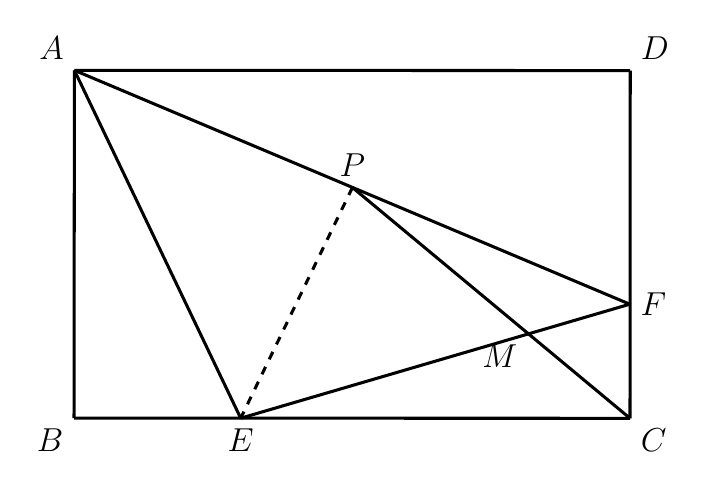
\begin{tikzpicture}[line width=1.1pt, line join=round]
  % Named coordinates (cm)
  \coordinate (A) at (-3.527,  2.210);
  \coordinate (D) at ( 3.532,  2.207);
  \coordinate (C) at ( 3.529, -2.209);
  \coordinate (B) at (-3.532, -2.207);
  \coordinate (E) at (-1.415, -2.208);
  \coordinate (F) at ( 3.526, -0.760);
  \coordinate (P) at ( 0.004,  0.722);
  \coordinate (M) at ( 2.235, -1.134);

  % Rectangle ABCD
  \draw (A) -- (B);
  \draw (B) -- (C);
  \draw (C) -- (D);
  \draw (D) -- (A);

  % Segments
  \draw (A) -- (F);      % passes through P
  \draw (A) -- (E);
  \draw (E) -- (F);
  \draw (P) -- (C);

  % Dashed segment
  \draw[dashed] (P) -- (E);

  % Labels
  \node[font=\fontsize{11.5}{13.8}\selectfont, above left]  at (A) {$A$};
  \node[font=\fontsize{11.5}{13.8}\selectfont, above right] at (D) {$D$};
  \node[font=\fontsize{11.5}{13.8}\selectfont, below left]  at (B) {$B$};
  \node[font=\fontsize{11.5}{13.8}\selectfont, below right] at (C) {$C$};
  \node[font=\fontsize{11.5}{13.8}\selectfont, below]       at (E) {$E$};
  \node[font=\fontsize{11.5}{13.8}\selectfont, right]       at (F) {$F$};
  \node[font=\fontsize{11.5}{13.8}\selectfont, above]       at (P) {$P$};
  \node[font=\fontsize{11.5}{13.8}\selectfont, below left]  at (M) {$M$};
\end{tikzpicture}
\end{document}